% Author: Izaak Neutelings (October 2020)
% Instructions: To compile, include data files from
%   https://github.com/IzaakWN/CodeSnippets/tree/master/LaTeX/TikZ/physics/dynamics_pendulum
% Other sources:
%   https://www.scielo.br/scielo.php?script=sci_arttext&pid=S1806-11172007000400024
%   https://www.researchgate.net/publication/262746594_Exact_solution_for_the_nonlinear_pendulum
%   https://tex.stackexchange.com/questions/545590/phase-portrait-of-van-der-pol-oscillator-with-pgfplots
%   http://matlab.cheme.cmu.edu/2011/08/09/phase-portraits-of-a-system-of-odes/
\documentclass[border=3pt,tikz]{standalone}
\usepackage{physics}
\usepackage{siunitx}
\sisetup{detect-all} % to allow \pi in \SI
\AtBeginDocument{\RenewCommandCopy\qty\SI}
\usepackage{tikz,pgfplots}
\usepackage[outline]{contour} % glow around text
\usetikzlibrary{calc}
\usetikzlibrary{angles,quotes} % for pic
\usetikzlibrary{arrows.meta}
\tikzset{>=latex} % for LaTeX arrow head
\contourlength{1.2pt}

\colorlet{xcol}{blue!70!black}
\colorlet{vcol}{green!60!black}
\colorlet{myred}{red!70!black}
\colorlet{myblue}{blue!70!black}
\colorlet{mygreen}{green!70!black}
\colorlet{mydarkred}{myred!70!black}
\colorlet{mydarkblue}{myblue!60!black}
\colorlet{mydarkgreen}{mygreen!60!black}
\colorlet{acol}{red!50!blue!80!black!80}
\tikzstyle{CM}=[red!40!black,fill=red!80!black!80]
\tikzstyle{xline}=[xcol,thick,smooth]
\tikzstyle{mass}=[line width=0.6,red!30!black,fill=red!40!black!10,rounded corners=1,
                  top color=red!40!black!20,bottom color=red!40!black!10,shading angle=20]
\tikzstyle{faded mass}=[dashed,line width=0.1,red!30!black!40,fill=red!40!black!10,rounded corners=1,
                        top color=red!40!black!10,bottom color=red!40!black!10,shading angle=20]
\tikzstyle{rope}=[brown!70!black,very thick,line cap=round]
\def\rope#1{ \draw[black,line width=1.4] #1; \draw[rope,line width=1.1] #1; }
\tikzstyle{force}=[->,myred,very thick,line cap=round]
\tikzstyle{velocity}=[->,vcol,very thick,line cap=round]
\tikzstyle{Fproj}=[force,myred!40]
\tikzstyle{myarr}=[-{Latex[length=3,width=2]},thin]
\def\tick#1#2{\draw[thick] (#1)++(#2:0.12) --++ (#2-180:0.24)}
\DeclareMathOperator{\sn}{sn}
\DeclareMathOperator{\cn}{cn}
\DeclareMathOperator{\dn}{dn}
\def\N{80} % number of samples in plots


\begin{document}


% PENDULUM
\def\L{2.8}  % string length
\def\ang{28} % angle string
\def\R{0.25} % ball radius
\def\F{1.0}  % force magnitude
\begin{tikzpicture}
  \message{^^JPendulum}
  \coordinate (M) at (\ang-90:\L);
  \coordinate (M') at (0,-\L);
  \coordinate (O) at (0,0);
  \coordinate (B) at (0,-\L-2.2*\R);
  \coordinate (FT) at ($(M)+(90+\ang:{\F*cos(\ang)+\R})$);
  \coordinate (FG) at ($(M)+(-90:{\F+\R})$);
  \coordinate (FGx) at ($(M)+(-90+\ang:{0.55*\F+\R})$);
  \coordinate (MA) at ($(M)+(180+\ang:{\F*sin(\ang)+\R})$);
  %\draw[faded mass] (M') circle(\R);
  \draw[<->] (M)++(\ang-32:0.2*\L) node[below right=-1,scale=0.9] {$x$}
    --++ (\ang:0.17*\L) --++ (90+\ang:0.17*\L) node[above right=-1,scale=0.9] {$y$};
  \draw[dashed] (O) -- (B);
  %\draw[dashed,myred!60!black] (MA) -- (FG);
  \draw[dashed,myred!60!black] (M) -- (FGx);
  \draw[dashed] (-90+\ang+10:\L) arc(-90+\ang+10:-110:\L) (B);
  \rope{(O) -- (M)} \path (O) -- (M) node[midway,above right=-1] {$L$};
  \fill[black] (O) circle(0.04);
  \draw[force] (M) -- (FT) node[midway,left=0] {$\vb{T}$};
  \draw[force] (M) -- (FG) node[right=0] {$m\vb{g}$};
  \draw[force,acol] (M) -- (MA) node[right=2,below=0] {$m\vb{a}$}; %{\contour{white}{$m\vb{a}$}};
  \draw[mass] (M) circle(\R) node {$m$};
  \draw pic[myarr,"$\theta$",xcol,draw=xcol,angle radius=22,angle eccentricity=1.30] {angle=B--O--M}; %_\text{max}
  \draw pic[myarr,"$\theta$",xcol,draw=xcol,angle radius=14,angle eccentricity=1.45] {angle=FG--M--FGx};
\end{tikzpicture}


% PENDULUM FORCES - ma
\begin{tikzpicture}
  \message{^^JPendulum forces}
  \def\F{1.4}  % force magnitude
  \coordinate (O) at (0,0);
  \coordinate (FT) at (90+\ang:{\F*cos(\ang)});
  \coordinate (FG) at (-90:\F);
  \coordinate (FGx) at (-90+\ang:{0.7*\F});
  \coordinate (MA) at (180+\ang:{\F*sin(\ang)});
  \draw[dashed,myred!60!black] (O) -- (FGx);
  \draw[dashed,myred!60!black] (MA) -- (FG);
  \draw[force] (O) -- (FT) node[midway,above right=-2] {$\vb{T}$};
  \draw[force] (O) -- (FG) node[right=0] {$m\vb{g}$};
  \draw[force,acol] (O) -- (MA) node[left=0] {$m\vb{a}$};
  \draw pic[myarr,"$\theta$",xcol,draw=xcol,angle radius=14,angle eccentricity=1.45] {angle=FG--O--FGx};
\end{tikzpicture}


% PENDULUM FORCES
\begin{tikzpicture}
  \message{^^JPendulum forces}
  \def\F{1.4}  % force magnitude
  \coordinate (O) at (0,0);
  \coordinate (FT) at (90+\ang:{\F*cos(\ang)});
  \coordinate (FG) at (-90:\F);
  \coordinate (FGx) at (-90+\ang:{\F*cos(\ang)});
  \coordinate (FGy) at (180+\ang:{\F*sin(\ang)});
  \draw[dashed,myred!60!black] (FGy) -- (FG); %-- (FGx);
  \draw[force] (O) -- (FT) node[midway,above right=-2] {$\vb{T}$};
  \draw[Fproj] (O) -- (FGy) node[pos=0.4,above left=-3,scale=0.86] {$mg\sin\theta$};
  \draw[Fproj] (O) -- (FGx) node[pos=0.5,above right=-3,scale=0.86] {$mg\cos\theta$};
  \draw[force] (O) -- (FG) node[right=0] {$m\vb{g}$};
  \draw pic[myarr,"$\theta$",xcol,draw=xcol,angle radius=14,angle eccentricity=1.45] {angle=FG--O--FGx};
\end{tikzpicture}


%% PENDULUM 
%\begin{tikzpicture}
%  \coordinate (M) at (0,-\L);
%  \coordinate (O) at (0,0);
%  \rope{(O) -- (M)} \path (O) -- (M) node[midway,above right=-2] {$L$};
%  \fill[black] (O) circle(0.04);
%  \draw[velocity] (M)++(-\R,0) --++ (-2.7*\R,0) node[above=0] {$\vb{v}$};
%  \draw[mass] (M) circle(\R) node {$m$};
%\end{tikzpicture}


% PHYSICAL PENDULUM
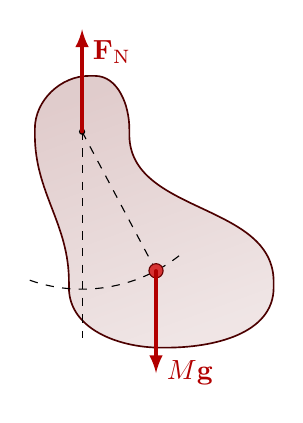
\begin{tikzpicture}
  \message{^^JPhysical pendulum}
  \def\L{2.0}  % string length
  \def\ang{28} % angle string
  \def\R{0.25} % ball radius
  \def\F{1.3}  % force magnitude
  \coordinate (M) at (\ang-90:\L);
  \coordinate (R) at (\ang-90:1.1*\L);
  \coordinate (M') at (0,-\L);
  \coordinate (O) at (0,0);
  \coordinate (B) at (0,-\L-2.5*\R);
  \coordinate (FT) at (90:\F);
  \coordinate (FG) at ($(M)+(-90:\F)$);
  \coordinate (FGx) at ($(M)+(-90+\ang:{0.55*\F+\R})$);
  \coordinate (MA) at ($(M)+(180+\ang:{\F*sin(\ang)+\R})$);
  \draw[mass]
    (180:0.3*\L) to[out=90,in=180] (80:0.36*\L) to[out=0,in=90] (0:0.3*\L) to[out=-90,in=90]
    ($(R)+(0:0.7*\L)$) to[out=-90,in=0] ($(R)+(-90:0.4*\L)$) to[out=180,in=-90] ($(R)+(-180:0.6*\L)$) to[out=90,in=-90] cycle; %node {$m$};
  \draw[dashed] (O) -- (B);
  \draw[dashed] (O) -- (M);
  %\draw[dashed,myred!60!black] (MA) -- (FG);
  \draw[dashed] (-90+\ang+10:\L) arc(-90+\ang+10:-110:\L) (B);
  \fill[black] (O) circle(0.04);
  \draw[CM] (M) circle(0.09);
  \draw[force] (O) -- (FT) node[below right=0] {$\vb{F}_\mathrm{N}$};
  \draw[force] (M) -- (FG) node[right=0] {$M\vb{g}$};
%  \draw[force,acol] (M) -- (MA) node[right=2,below=0] {$m\vb{a}$}; %{\contour{white}{$m\vb{a}$}};
%  \draw pic[myarr,"$\theta$",xcol,draw=xcol,angle radius=22,angle eccentricity=1.30] {angle=B--O--M}; %_\text{max}
%  \draw pic[myarr,"$\theta$",xcol,draw=xcol,angle radius=14,angle eccentricity=1.45] {angle=FG--M--FGx};
\end{tikzpicture}



% PENDULUM EQUATIONS - CLOSED TRAJECTORIES
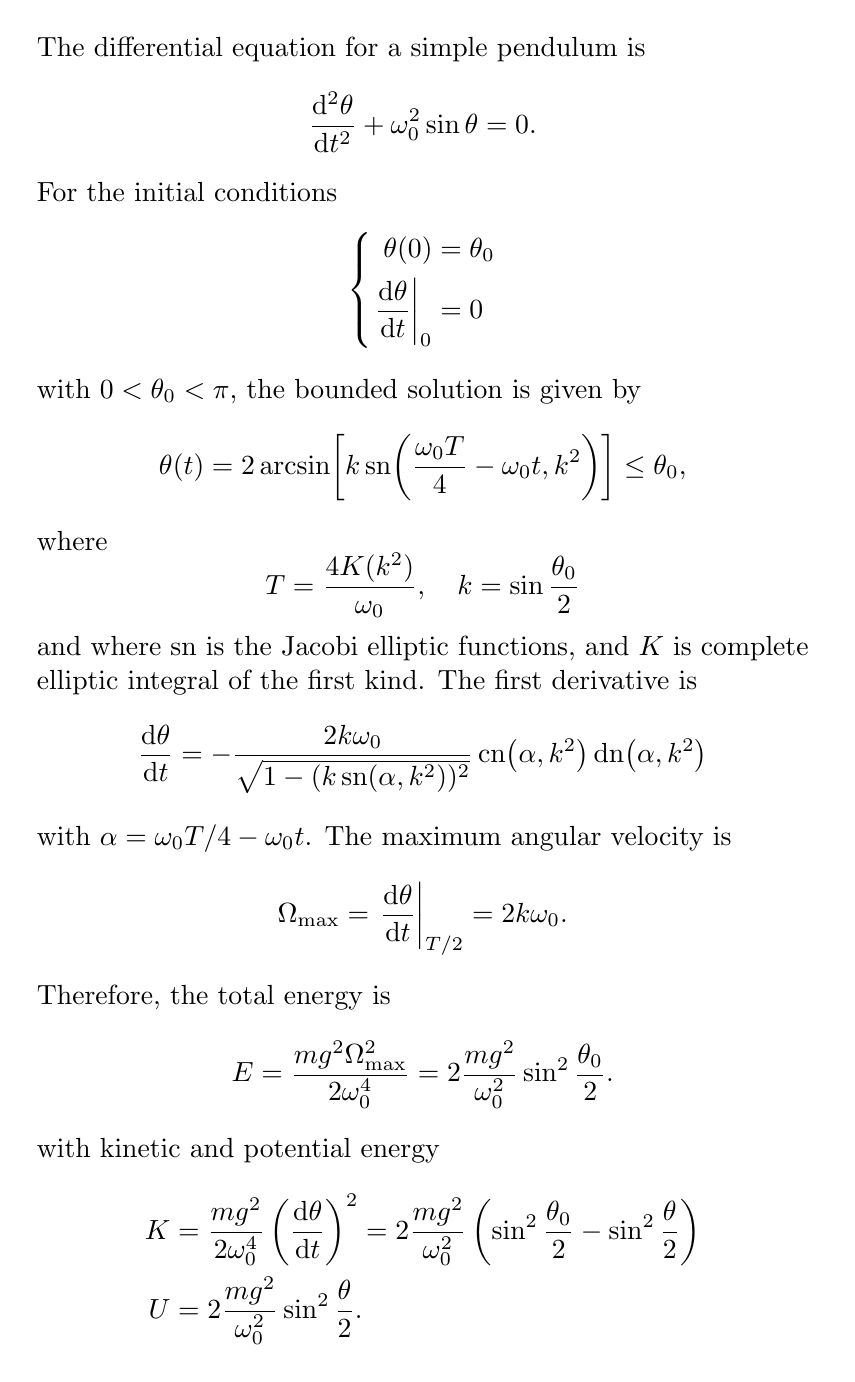
\begin{tikzpicture}[scale=1]
  \message{^^JPendulum equations (closed/bounded)}
  \def\myarg{\left(\alpha,k^2\right)}
  \node[align=left] at (0,0) {
    \begin{minipage}{9.8cm}
      The differential equation for a simple pendulum is
      \begin{equation*}
        \dv{^2\theta}{t^2} + \omega_0^2\sin\theta = 0.
      \end{equation*}
      For the initial conditions
      \begin{equation*}
        \left\{\begin{aligned}
          \theta(0) &= \theta_0\\
          \left.\dv{\theta}{t}\right|_{0} &= 0
        \end{aligned}\right.
      \end{equation*}
      with $0<\theta_0<\pi$,
      the bounded solution is given by
      \begin{equation*}
        \theta(t)
        = 2\arcsin\!\left[k\sn\!\left(\frac{\omega_0T}{4}-\omega_0t,k^2\right)\right]
        \leq \theta_0,
      \end{equation*}
      where
      \begin{equation*}
        %0<\theta_0<\pi,\quad
        T = \frac{4K(k^2)}{\omega_0},\quad
        k = \sin{\frac{\theta_0}{2}}
      \end{equation*}
      and where $\sn$ is the Jacobi elliptic functions,
      and $K$ is complete elliptic integral of the first kind.
      The first derivative is
      \begin{equation*}
        \dv{\theta}{t}
        = -\frac{2 k \omega_0}{\sqrt{1-(k \sn\!\myarg)^2}} \cn\!\myarg\dn\!\myarg
      \end{equation*}
      with $\alpha = \omega_0T/4-\omega_0t$.
      %\begin{equation*}
      %  \alpha = \frac{\omega_0T}{4}-\omega_0t.
      %\end{equation*}
      The maximum angular velocity is
      \begin{equation*}
        \Omega_\mathrm{max} = \left.\dv{\theta}{t}\right|_{T/2} = 2k\omega_0.
      \end{equation*}
      Therefore, the total energy is
      \begin{equation*}
        E = \frac{mg^2\Omega_\mathrm{max}^2}{2\omega_0^4}
          = 2\frac{mg^2}{\omega_0^2}\sin^2\frac{\theta_0}{2}.
      \end{equation*}
      with kinetic and potential energy
      \begin{align*}
        K &= \frac{mg^2}{2\omega_0^4}\left(\dv{\theta}{t}\right)^2
           = 2\frac{mg^2}{\omega_0^2}\left( \sin^2\frac{\theta_0}{2} - \sin^2\frac{\theta}{2} \right) \\
        U &= 2\frac{mg^2}{\omega_0^2}\sin^2\frac{\theta}{2}.
      \end{align*}
     \end{minipage}
  };
\end{tikzpicture}


% PENDULUM EQUATIONS - OPEN TRAJECTORIES
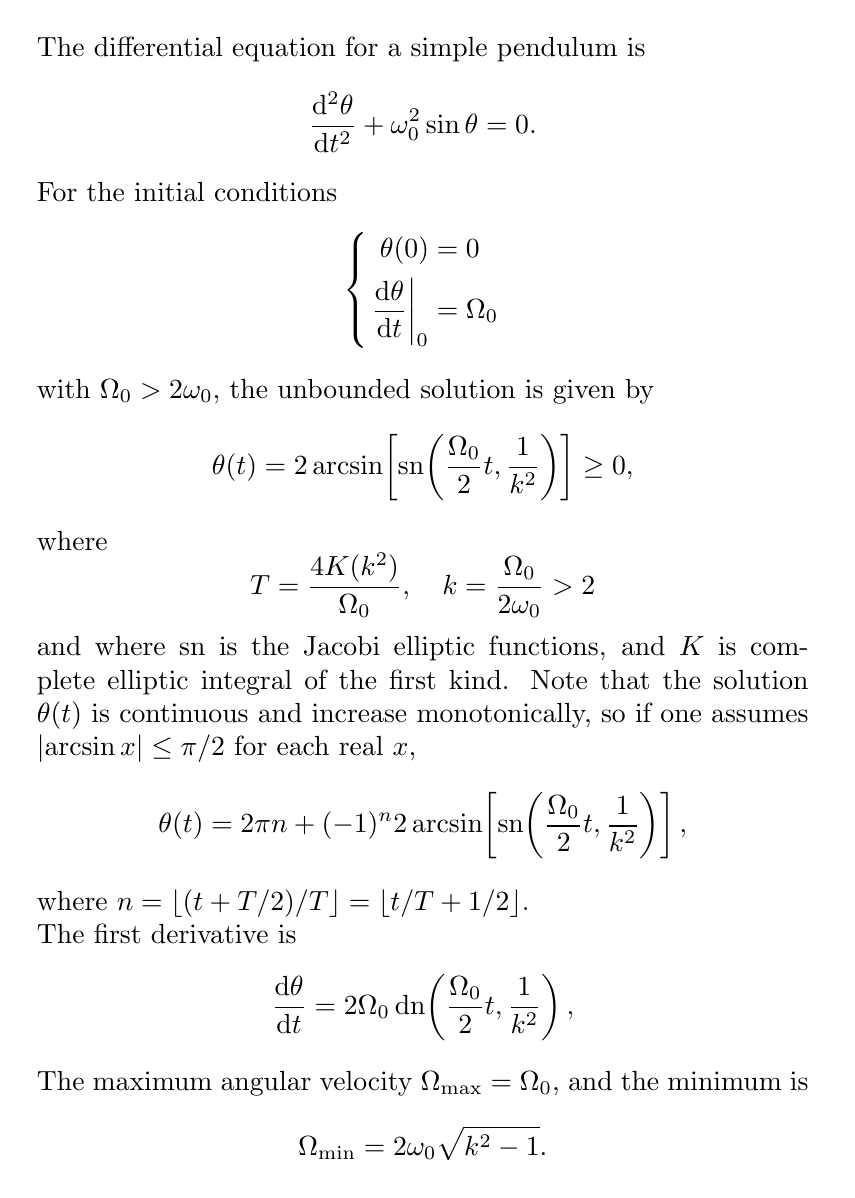
\begin{tikzpicture}[scale=1]
  \message{^^JPendulum equations (open/unbounded)}
  \def\myarg{\left(\frac{\Omega_0}{2}t,\frac{1}{k^2}\right)}
  \node[align=left] at (0,0) {
    \begin{minipage}{9.8cm}
      The differential equation for a simple pendulum is
      \begin{equation*}
        \dv{^2\theta}{t^2} + \omega_0^2\sin\theta = 0.
      \end{equation*}
      For the initial conditions
      \begin{equation*}
        \left\{\begin{aligned}
          \theta(0) &= 0 \\
          \left.\dv{\theta}{t}\right|_{0} &= \Omega_0 %> 2\omega_0
        \end{aligned}\right.
      \end{equation*}
      with $\Omega_0 > 2\omega_0$,
      the unbounded solution is given by
      \begin{equation*}
        \theta(t)
        = 2\arcsin\!\left[\sn\!\myarg\right]
        \geq 0,
      \end{equation*}
      where
      \begin{equation*}
        %\Omega_0 > 2\omega_0,\quad
        T = \frac{4K(k^2)}{\Omega_0},\quad
        k = \frac{\Omega_0}{2\omega_0} > 2
      \end{equation*}
      and where sn is the Jacobi elliptic functions,
      and $K$ is complete elliptic integral of the first kind.
      Note that the solution $\theta(t)$ is continuous and increase monotonically,
      so if one assumes $\abs{\arcsin x}\leq\pi/2$ for each real $x$,
      \begin{equation*}
        \theta(t)
        = 2\pi n + (-1)^n 2\arcsin\!\left[\sn\!\myarg\right],
      \end{equation*}
      where $n=\lfloor(t+T/2)/T\rfloor=\lfloor t/T+1/2\rfloor$.\\
      The first derivative is
      \begin{equation*}
        \dv{\theta}{t} = 2\Omega_0\dn\!\myarg,
      \end{equation*}
      The maximum angular velocity $\Omega_\mathrm{max}=\Omega_0$,
      and the minimum is
      \begin{equation*}
        \Omega_\mathrm{min} = 2\omega_0\sqrt{k^2-1}.
      \end{equation*}
    \end{minipage}
  };
\end{tikzpicture}


\end{document}